\section{Experiments}
\label{sec:experiments}
\subsection{Experimental set-up}
We implemented \provalg\ in Java 8 using PostgreSQL 9.6.3 as the underlying DBMS. All experiments were conducted
on a Linux server \eat{Distribution? (Gianmaria)}with an Intel(R) Xeon(R) CPU E5-2630 v4 @ 2.20GHz and 64GB of central memory. \eat{claim the use of code from CoreCover algorithm and provide the link to our own code}

{\bf Datasets.} %Three datasets were used in the experiments.
Two realistic datasets were used in addition to GENCODE: 
Hetionet\footnote{\url{https://neo4j.het.io/browser/}} and DBLP-NSF\footnote{\url{https://data.mendeley.com/datasets/ycnngyv5bd}}. 
Summary information of the three datasets, including the number of relations, average size per relation, and the size of the largest relation is presented in Table \ref{Table: datasets_summary}.

We converted Hetionet, which is stored in Neo4j, into a relational database\footnote{Available at 
\url{https://github.com/thuwuyinjun/Data_citation_provenance/files/2417454/hetionet_postgresql.zip}}.
% \scream{Should also make relational representation of Hetionet available.}
% Hetionet aims at building network to systematically identify why drugs work and predict new therapies for drugs. It connects some previously isolated information such as genes, drugs as well as biological processes in which drugs and genes may involve.
DBLP-NSF was developed by the authors of \cite{wu2018data}, and integrates DBLP publication information with NSF award information to augment traditional paper citations with funding information.

\begin{table}
\centering
\caption{Summary of datasets}
\small
\begin{tabular}[!h]{|>{\centering\arraybackslash}p{2cm}|>{\centering\arraybackslash}p{1.5cm}|>{\centering\arraybackslash}p{2cm}|>{\centering\arraybackslash}p{2cm}|} \hline
Dataset name& relation \# &average tuple \# per relation& tuple \# of largest relation \\ \hline
GENECODE&7&600k&2000k \\ \hline
Hetionet&38&60k&500k \\ \hline
DBLP-NSF&17&600k&6000k \\ \hline
\end{tabular}
\label{Table: datasets_summary}
\end{table}


{\bf Workloads.} 
We test the performance of \provalg\ using both {\em synthetic} and {\em realistic} workloads. As mentioned earlier,  one essential step for aggregate views is to compare the provenance of views and queries. In order to retrieve the provenance of views, we can use either {\em eager} or {\em lazy} strategy.  We compare these two strategies using both forms of workloads. The performance also depends on the {\em policies}. As mentioned in Section \ref{Sec: implementation}, different policies can lead to different results, and can generate either all or some of the covering sets. Due to space limitations, only the case where the all the covering sets are generated is presented here\eat{do we need to call it full case}.

%only care about t_cs
The purpose of using {\em synthetic workloads} is to determine the key factors which influence performance. 
Extensive experiments were performed in~\cite{wu2018data} measuring the \textit{total reasoning time}  to generate the covering sets ($t_{cs}$)
 and the \textit{citation generation time}   after covering sets are constructed ($t_{cg}$).  The \textit{citation generation time} ($t_{cg}$) is not considered here since \provalg\ only changes how {\em valid view mappings} are determined during covering sets construction process %(rather than {\em formatted citations}) 
relative to the implementations of \rba. % in~\cite{wu2018data}.


%what key factors can influence the performance
%In terms of $t_{cs}$, based on the experimental results reported in \cite{wu2018data}, 
\eat{Maybe put in a table with these abbreviations in case people forget?}
In \cite{wu2018data}, $t_{cs}$ primarily depends on: 1) the number of view mappings (denoted $N_v$); 2) the total number of predicates under the view mappings (denoted $N_p$); 3) the size of the query instance before duplicates are removed (which is the same as the total number of how-provenance monomials in the query instance $N_{pq}$). The experiments measure the effect of these metrics on $t_{cs}$. %Plus, according to the brief time complexity analysis in Section \ref{Sec: implementation}, 
The total number of how-provenance monomials in the view instance on average ($N_{pv}$) can influence performance according to the analysis in Section \ref{Sec: implementation}, and is also considered in the experiments.

%compare to TLA/SSLA
The trade-offs between \provalg\ and two implementations of the \rba\ proposed in \cite{wu2018data}, TLA and SSLA, are also  measured. 
% We do not consider the {\em pure view-based approach} of \cite{wu2018data},\scream{maybe not correct} since this does not generate fine-grained citations. %;  it is not difficult to extend the view-based approach to handle aggregate queries using conjunctive views. 
As mentioned before, \rba\ can be extended to handle aggregate queries when views are conjunctive views (but not aggregate views). In this case, TLA, SSLA and \provalg\ all generate the same final, fine-grained citations.
%, which derives us to conduct experiments in this setting.

% Plus, according to the complexity analysis in Section \ref{Sec: implementation}, the time to generate covering sets ($t_{cs}$) should also depend on the total number of how-provenance monomials in query and view instance (denoted $N_{pq}$ and $N_{pv}$ respectively) when the views are aggregate views while queries are aggregate queries, which is also experimentally verified herein.

In the {\em realistic workloads}, we use frequent queries against the three databases, and build views to represent the portions of data in the database associated with predefined citations. Complete details of  the views and queries used are available in our Github repository\footnote{\url{https://github.com/thuwuyinjun/Data_citation_provenance}}. 

To mimic the summary information provided by GENCODE, we defined aggregate views to compute the total number of transcripts per gene, and total number of exons per gene and per transcript. Two additional parameterized views are also defined to represent basic information (e.g. ID, name and type) for each transcript and gene, respectively. The realistic queries  compute the total number of exons ($q1$) and the total number of transcripts per type of gene ($q2$) respectively.

For DBLP-NSF we use the realistic views defined in \cite{wu2018data}. We also add aggregate views to reflect publicly available statistics related to this database, such as the total number of publications per faculty member\footnote{\url{http://csrankings.org/}} and total number of grants per institution\footnote{\url{https://dellweb.bfa.nsf.gov/awdlst2/default.asp}}. Some realistic aggregate queries are designed to represent other summary information, such as total number of publications per institute ($q3$) and total amount of grants per state ($q4$).

Hetionet integrates information from various resources, and includes information about genes, biological process, drugs etc.  This information is stored in different relations in the database. Of these, the biological process relation is associated with citation information (i.e. related publication IDs). After consulting with the authors of Hetionet, two views were defined. The first one is a parameterized view showing the  biological processes that a particular gene is involved in. The second counts the total number of connections between each biological process and corresponding genes by joining several relations, such as the biological process and gene relations.  A typical query ($q5$) counts the total number of connections between each biological process and a certain drug via some genes.


\begin{table}
\centering
\caption{Notation used in the experiments}
\small
\begin{tabular}[!h]{|c|>{\centering\arraybackslash}p{6.8cm}|} \hline
Notation & Meaning \\ \hline
$t_{cs}$&total reasoning time to generate the covering sets for all query tuples \\ \hline
$t_{cg}$&citation generation time after covering sets are constructed \\ \hline
$N_v$&total number of view mappings \\ \hline
$N_p$&total number of predicates under the view mappings \\ \hline
$N_{pq}$&total number of how-provenance monomials in the query instance \\ \hline
$N_{pv}$&total number of how-provenance monomials in the view instance on average\\ \hline
\end{tabular}
\label{Table: notation_summary}
\end{table}

\begin{figure*}
\captionsetup[subfigure]{width=1\textwidth}
     \centering
    \begin{subfigure}{0.30\textwidth}
    \hspace*{-0.8cm}
        \raisebox{-\height}{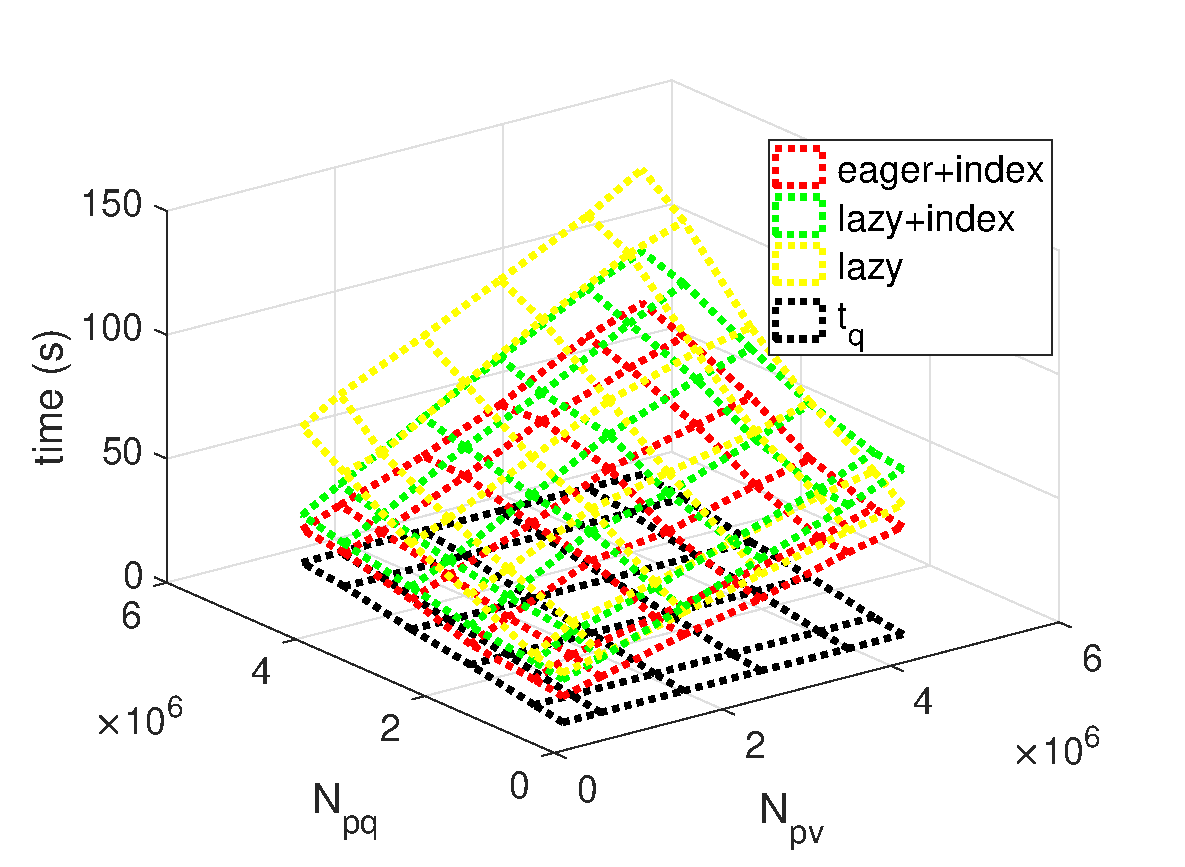
\includegraphics[height = 0.8\textwidth, width=1.2\textwidth]{Figures/synthetic_instance_size.eps}}
        \caption{$t_{cs}$ with varied $N_{pq}$ and $N_{pv}$}     \label{fig:stress_test_instance_size}
    \end{subfigure}
    \hfill
    \begin{subfigure}{0.30\textwidth}
    \hspace*{-0.8cm}
        \raisebox{-\height}{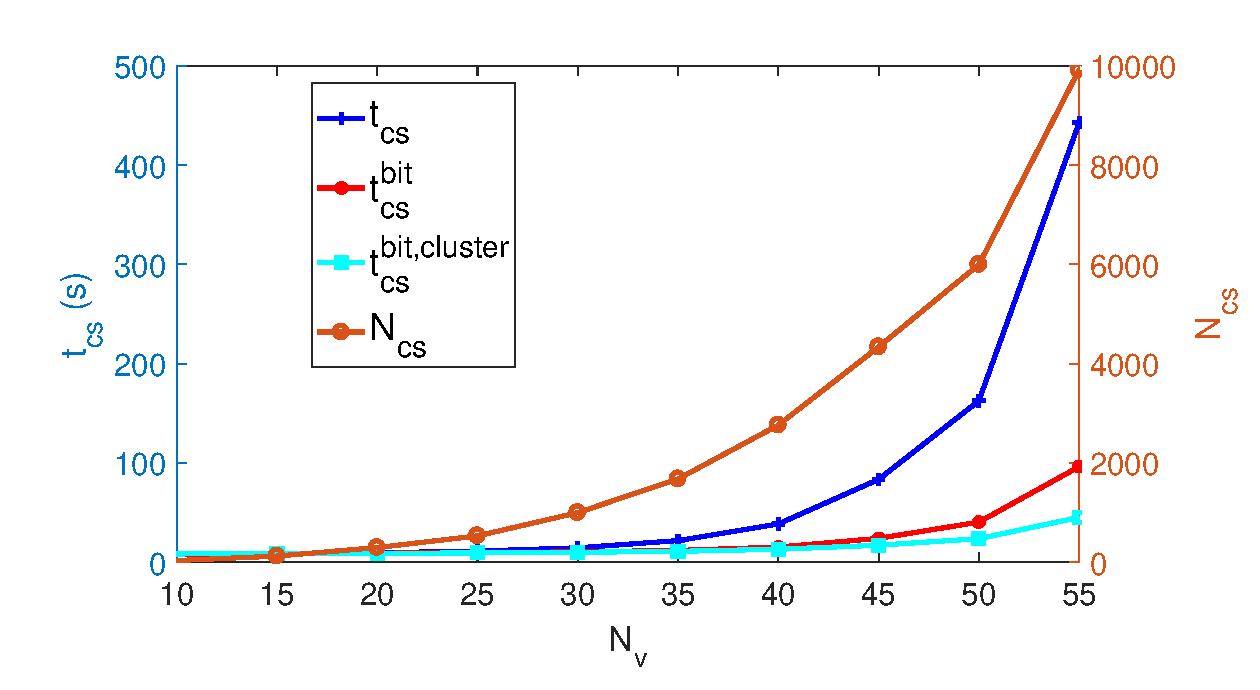
\includegraphics[height = 0.8\textwidth, width=1.2\textwidth]{Figures/synthetic_view_num.eps}}
        \caption{$t_{cs}$ with varied $N_v$}
        \label{fig:stress_test_view_num}
    \end{subfigure}
    \hfill
    \begin{subfigure}{0.30\textwidth}
    \hspace*{-0.8cm}
        \raisebox{-\height}{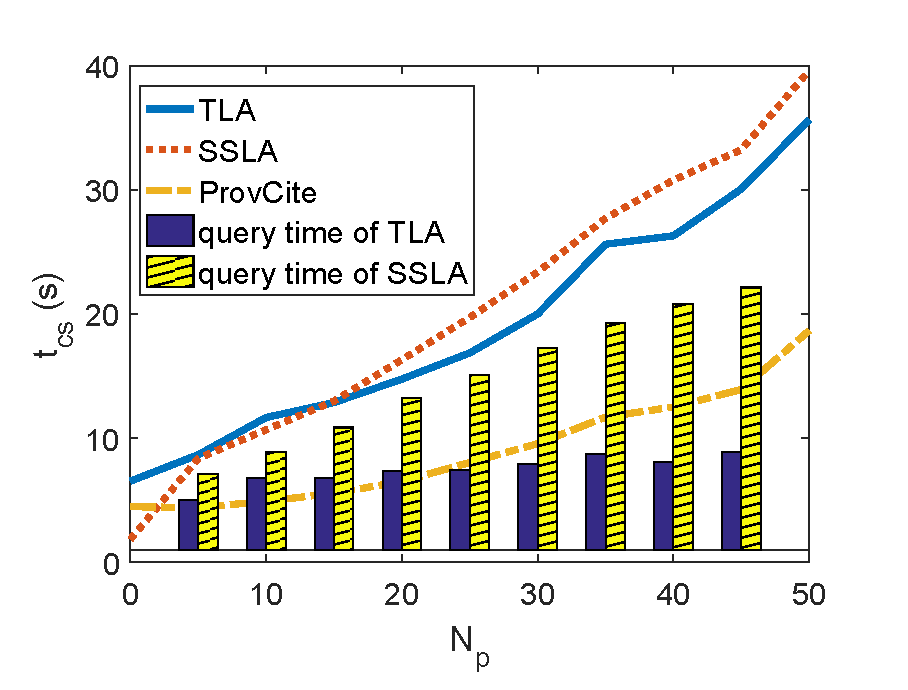
\includegraphics[height = 0.8\textwidth, width=1.2\textwidth]{Figures/synthetic_predicate_num.eps}}
        \caption{$t_{cs}$ with varied $N_p$}
        \label{fig:stress_test_predicate_num_time}
    \end{subfigure}
    \caption{Experimental results for synthetic workloads}
\end{figure*}

Table \ref{Table: notation_summary} provides a summary of the notation defined in this subsection.% which will be used in the remainder of this section.

\subsection{Experimental results}
We now report on results from the synthetic and realistic workloads.

\subsubsection{Synthetic workloads} 
We measured the impact of the size of provenance in both the query and view instances on time performance (Exp1), and the relative performance of \provalg\ and two implementations of the \rba, i.e. TLA and SSLA while varying the number of view mappings (Exp2) and number of view predicates (Exp3).

\textbf{Exp1.}  This experiment measures how the total reasoning time $t_{cs}$ is influenced by the total number of how-provenance monomials in the query instance ($N_{pq}$) as well as 
%the total number of how-provenance monomials 
in the view instance ($N_{pv}$). We randomly generate an aggregate query, and vary $N_{pq}$ by adding appropriate predicates. A fixed number of aggregate views are also generated such that there is exact one view mapping from each of them to the query and the total number of view mappings is fixed at 10, which is a reasonable number in practice. Both $N_{pq}$ and $N_{pv}$ are varied from 50K to 1M. $t_{cs}$ is measured for different ($N_{pq}$, $N_{pv}$) pairs under both the {\em eager} and {\em lazy} strategy.  

\textbf{Results.} 
The time performance, $t_{cs}$, is shown using 3D surfaces in Figure \ref{fig:stress_test_instance_size}, with the eager strategy shown in blue and the lazy strategy shown in red. It shows that the time performance under the eager strategy is only slightly better  than under the lazy strategy (10\% - 40\% faster). In the worst case, in which both $N_{pv}$ and $N_{pq}$ are 1 million, it takes no more than 150 seconds. This case will be rare, so the performance in practice should be much better. We also measured the extra space needed for the eager strategy, where the provenance of views is precomputed and stored in the database; it takes about 180 MB in the database to store the provenance for each view when the instance of the view includes up to 1 million how-provenance monomials. 

\textbf{Exp2.} The goal of this experiment is to compare the relative performance of \provalg, TLA and SSLA while varying the number of view mappings ($N_v$).
\eat{We call the system \provalg\ in the title, it is inconsistent to call it Prov here. I guess system is called \provalg\ while the algorithm is called Prov??}Since TLA and SSLA cannot handle aggregate views, only conjunctive views are used. So there is no difference between {\em eager} and {\em lazy} strategy since the provenance of views is not necessary. The query is a fixed aggregate query, with 500k how-provenance monomials in its instance. $N_v$ is varied from 1 to 50 and there are no predicates or lambda variables for each individual view. 

\textbf{Results.}
The experimental results are presented in Figure \ref{fig:stress_test_view_num}, which shows that $t_{cs}$ grows rapidly with the increasing number of view mappings ($N_v$) for all the three approaches. This is due to the fact that an exponential  number of covering sets are generated, which is inevitable. It is worth noting that \provalg\ \textit{outperforms} TLA when $N_v < 40$, and is on par with SSLA until $N_v >30$.
Furthermore it only adds a little extra overhead when $N_v > 40$ compared to the competitors. 


\textbf{Exp3.} In this experiment, \provalg\ is compared with TLA and SSLA while varying the total number of predicates ($N_p$) in views. Similar to Exp2, the query is an aggregate query which can generate about 500k tuples. The number of view mappings is fixed at 10 and there are initially no predicates. At each run, one more local predicate is added. As shown in \cite{wu2018data}, increasing $N_p$ can significantly influence the performance of TLA and SSLA by 1) increasing the query time since the query is extended to explicitly evaluate the satisfiability of predicates of the views in the query instance; 2) increasing the number of {\em reasoning groups} since we need to compute covering sets for each group and thus more {\em reasoning groups} in the query instance means more reasoning time. In theory, \provalg\ will also suffer from a large number of groups but will save on query time.

\textbf{Results.} The experimental results are shown in Figure \ref{fig:stress_test_predicate_num_time}, which matches the analysis above. As the number of predicates increases, $t_{cs}$ 
increases slowly for \provalg. In contrast, TLA and SSLA are twice as slow as \provalg\ for large $N_p$. To understand the reason for this, the query time for TLA and SSLA is also presented in this figure, which implies that the increasing query time becomes the major overhead for both TLA and SSLA, thus slowing down the computation.

{\bf Discussion.} The experiments reveal that all four metrics, $N_{pq}$ (the total number of how-provenance monomials in the query instance), $N_{pv}$ (the total number of how-provenance monomials in the view instance on average), $N_v$ (the total number of view mappings), $N_p$ (the total number of predicates under the view mappings) can affect the total reasoning time $t_{cs}$. In extreme cases, where the value of the metric is very large, bad performance is unavoidable.  However these cases are unlikely to happen in practice. We therefore expect reasonable time performance for realistic workloads. 

In the case of aggregate views where how-provenance is necessary, the  eager strategy beats the lazy strategy in terms of time.  The speedup is small (10\%-40\%), however, extra space is needed (up to 180 MB per view). So in practice, the choice between the eager or lazy strategy depends on whether speed or space is more important. In comparison to the previous approaches, TLA and SSLA, \provalg\ is not only more powerful in that it supports aggregate views but is also (surprisingly) frequently more efficient.  

\subsubsection{Realistic workloads}
\label{ssec: realistic}
The experimental results for realistic workloads are presented in Table \ref{Table: realistic_performance}, which includes the time to generate covering sets ($t_{cs}$) for both the lazy and eager strategies, as well as the metrics that can potentially affect the performance: the total number of how-provenance monomials in the query instance ($N_{pq}$), the total number of view mappings ($N_v$), the total number of predicates in the views under all the view mappings ($N_p$) and the query time to simply generate instance. Except for $q1$, most of $t_{cs}$ is less than 10 seconds for all queries. Although $N_{pq}$ is more than one million in $q1$, the total reasoning time ($t_{cs}$) is only about a half minute under both strategies, which is an acceptable considering the large query instance. To see how this compares to simply generating the query output, we list the query running time in the last column. When users are browsing the query result, the system can generate covering sets for all query tuples in the back-end, ready to instantly construct formatted citations when users select tuples of interest.

\eat{Comparing to time to simply generate query instance (See last column), $t_{cs}$ is still reasonable considering the large instance. When users are browsing the query result, the system can generate covering sets for all query tuple in the back-end, ready to construct formatted citations when users select tuples of interest.}

{\bf Discussion.} The experimental results above show that reasonable time performance can be guaranteed in practice where none of the crucial metrics become too large.  Revisiting the experimental results for synthetic workloads, when the total number of how-provenance monomials in the query instance ($N_{pq}$) is more than 1 million (as in $q1$), the reasoning time ($t_{cs}$) can be large (up to 150 seconds). However, the time shown for $q1$ is significantly smaller since the number of view mappings ($N_v$) is only 1, and the reasoning time relies on both $N_v$ and $N_{pq}$.




\begin{table}
\centering
\caption{Experimental results on realistic datasets}
\small
\begin{tabular}[!h]{|>{\centering\arraybackslash}p{0.8cm}|>{\centering\arraybackslash}p{1cm}|>{\centering\arraybackslash}p{1cm}|>{\centering\arraybackslash}p{1cm}|>{\centering\arraybackslash}p{0.25cm}|>{\centering\arraybackslash}p{0.25cm}|>{\centering\arraybackslash}p{1.5cm}|} \hline
Query& $t_{cs}$ (s) (eager) & $t_{cs}$ (s) (lazy)& $N_{pq}$&$N_v$&$N_p$&query time (s) \\ \hline
$q1$&22.51s&36.84s&1237914&1&0&1.02 \\ \hline
$q2$&4.40s&6.03s&203835&2&0&0.13 \\ \hline
$q3$&8.47s&11.23s&507515&2&0&1.15 \\ \hline
$q4$&3.72s&5.68s&416716&1&0&0.67\\ \hline
$q5$&4.56s&6.82s&243901&3&0&0.51 \\ \hline
\end{tabular}
\label{Table: realistic_performance}
\end{table} 


